\chapter{Ferramentas de suporte}
\label{chapter:suporte}

\section{Introdução}

A adoção de uma mão robótica \textit{open-source} apresenta diversas vantagens, entre as quais se destacam a disponibilização de código de apoio e a existência de decisões previamente fundamentadas relativamente à seleção de componentes mecânicos e eletrónicos. Estas características permitem reduzir significativamente o tempo necessário para o desenvolvimento de um sistema funcional, evitando o esforço associado ao desenho e especificação de soluções desde a parte inicial do projeto. 

Neste capítulo, descrevem-se os principais elementos já existentes e utilizados como base no presente trabalho, com particular destaque na LEAP Hand, desenvolvida por Shaw, et al. \cite{shaw2023leaphand}. Serão abordadas as escolhas efetuadas por estes autores ao nível dos motores, do controlador de motores, da fonte de alimentação e das ferramentas de software disponibilizadas, que serviram de ponto de partida para o desenvolvimento realizado neste projeto.

\section{Hardware}

\subsection{Motores Dynamixel}

No desenvolvimento da LEAP Hand, Shaw, et al. \cite{shaw2023leaphand} optaram por utilizar os motores Dynamixel XC330-M288-T, amplamente utilizados em aplicações robóticas devido à sua fiabilidade, eficiência energética e dimensões compactas. Estes atuadores oferecem controlo detalhado sobre posição, velocidade e corrente, permitindo gerar movimentos suaves, reproduzíveis e bem definidos — uma característica fundamental em sistemas de manipulação, como mãos robóticas antropomórficas. 

Os motores Dynamixel XC330-M288-T (Figura \ref{fig:motor}) operam a 5V e apresentam uma corrente nominal de 1.8A, o que os torna compatíveis com fontes de alimentação de baixa potência, mantendo um desempenho consistente. Adicionalmente, a comunicação digital via protocolo TTL permite a ligação e controlo eficiente de múltiplos motores em rede, facilitando a sua integração com microcontroladores e promovendo uma arquitetura modular e escalável.

\begin{figure}[H]
    \centering
    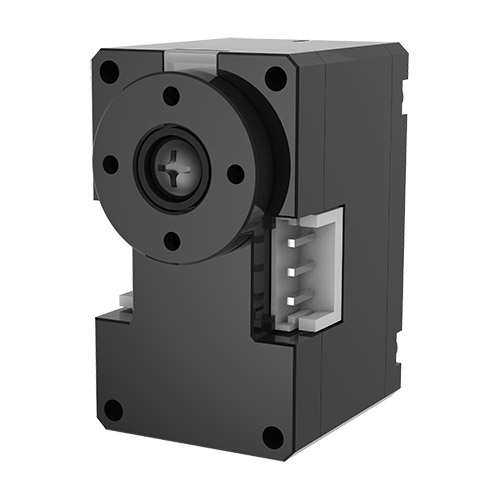
\includegraphics[height=6cm]{figs/chapter3/motor.jpg}
    \caption{Motor Dynamixel XC330-M288-T utilizado na construção da LEAP Hand\cite{shaw2023leaphand} }
    \label{fig:motor}
    
\end{figure}

O controlo destes motores pode ser realizado por diferentes meios, nomeadamente através da ferramenta gráfica Dynamixel Wizard 2.0, útil para configuração e diagnóstico, e da biblioteca Dynamixel SDK, que permite o controlo programático e a integração com sistemas desenvolvidos em diversas linguagens de programação. Estas opções tornam o sistema versátil e facilmente adaptável a diferentes contextos de desenvolvimento, incluindo ambientes compatíveis com \ac{ROS}.

Os motores Dynamixel armazenam e gerem os seus parâmetros internos através de uma tabela de controlo de memória, onde cada parâmetro — como posição, velocidade, corrente ou temperatura — está associado a um endereço específico. Essa tabela encontra-se dividida em duas secções principais: a \textbf{EEPROM}, que contém parâmetros permanentes (como o ID do motor, taxa de transmissão, limites de corrente ou posição) e só pode ser modificada após a reinicialização do motor; e a \textbf{RAM}, onde se encontram os parâmetros dinâmicos, como a posição atual, velocidade, temperatura e estado do motor, permitindo atualizações em tempo real durante a operação. Esta estrutura torna o controlo dos motores altamente flexível e eficiente, uma vez que permite o acesso direto e segmentado aos dados necessários para a gestão do comportamento do sistema robótico.

\subsection{Controlador e Fonte de Alimentação}

Para além da seleção dos motores, a escolha do controlador de comunicação e da fonte de alimentação tem um impacto significativo no desempenho e na fiabilidade do sistema. No que respeita à interface de comunicação com os motores, os autores da LEAP Hand \cite{shaw2023leaphand} optaram por utilizar o \textbf{Dynamixel U2D2} (Figura \ref{fig:u2d2}), um conversor USB para TTL \textit{half-duplex}.  Este dispositivo permite estabelecer comunicação entre um computador e múltiplos motores Dynamixel através de uma única porta serial, utilizando um barramento em cadeia (\textit{daisy chain}). Este método de ligação, possível graças à arquitetura \textit{half-duplex} dos motores, permite que vários atuadores sejam ligados em série, reduzindo significativamente a complexidade do sistema e facilitando a sincronização entre motores. O U2D2 suporta taxas de transmissão elevadas (até 4,5 Mbps), possui um conector JST de 3 pinos para comunicação TTL, e inclui um terminal de alimentação auxiliar (VDD), permitindo a alimentação dos motores a partir de uma fonte externa apropriada. 

Relativamente à fonte de alimentação, foi necessário considerar que cada motor Dynamixel XC330-M288-T pode atingir um consumo máximo de 1.8A em condições de carga. Tendo em conta a utilização de 16 motores, a corrente total exigida pode atingir os 28.8A. Assim, foi selecionada uma fonte de alimentação industrial (Figura \ref{fig:fonte}) com saída estabilizada de 5V — a mesma tensão nominal dos motores — e capacidade de fornecimento de até 30A, assegurando uma margem de segurança adequada para o funcionamento simultâneo de todos os atuadores.

\begin{figure}[H]
    \centering
    \begin{minipage}[b]{0.45\textwidth}
        \centering
        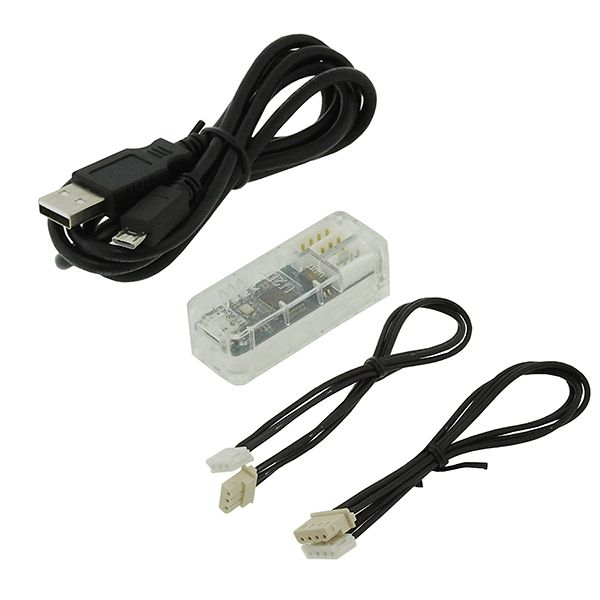
\includegraphics[width=\textwidth]{figs/chapter3/u2d2.jpg}
        \caption{Controlador Dynamixel U2D2 utilizado para controlar os motores do projeto}
        \label{fig:u2d2}
    \end{minipage}
    \hfill
    \begin{minipage}[b]{0.45\textwidth}
        \centering
        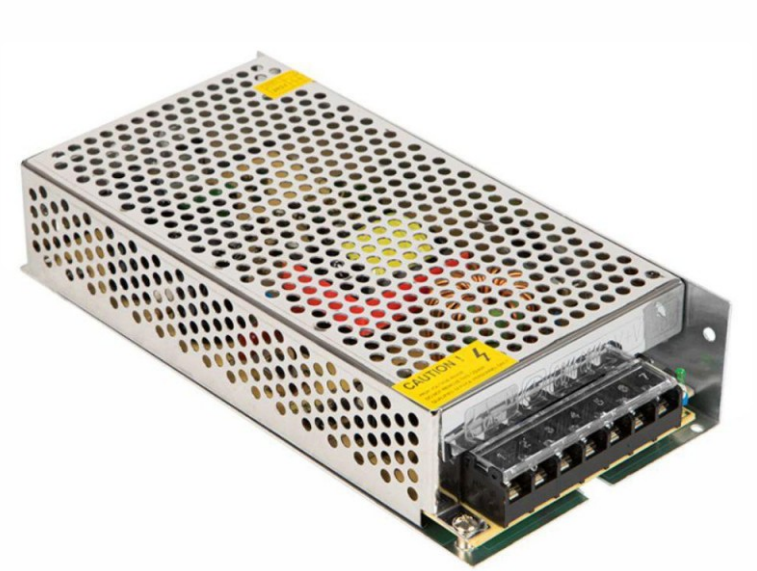
\includegraphics[width=\textwidth]{figs/chapter3/fonte.png}
        \caption{Fonte de Alimentação industrial com saída a 5V e capacidade de 30A utilizada neste projeto}
        \label{fig:fonte}
    \end{minipage}
\end{figure}


\section{Software}

\subsection{Dynamixel Wizard 2.0}

A Dynamixel disponibiliza diversas ferramentas para configuração, monitorização e controlo dos seus motores, entre as quais se destaca o Dynamixel Wizard 2.0, uma interface gráfica intuitiva (Figura \ref{fig:dynamixel_wizard}) que permite ao utilizador interagir diretamente com cada motor. Antes de iniciar o controlo coordenado de um sistema com múltiplos atuadores, é essencial garantir que cada motor possui um identificador único. Por defeito, todos os motores Dynamixel são fornecidos com o mesmo identificador (ID = 1), o que inviabiliza a sua utilização simultânea num mesmo barramento de comunicação. Assim, uma das primeiras tarefas consiste na atribuição de um ID exclusivo a cada motor, procedimento que pode ser facilmente realizado através do Dynamixel Wizard 2.0, modificando o parâmetro correspondente no firmware do atuador.


\begin{figure}[H]
    \centering
    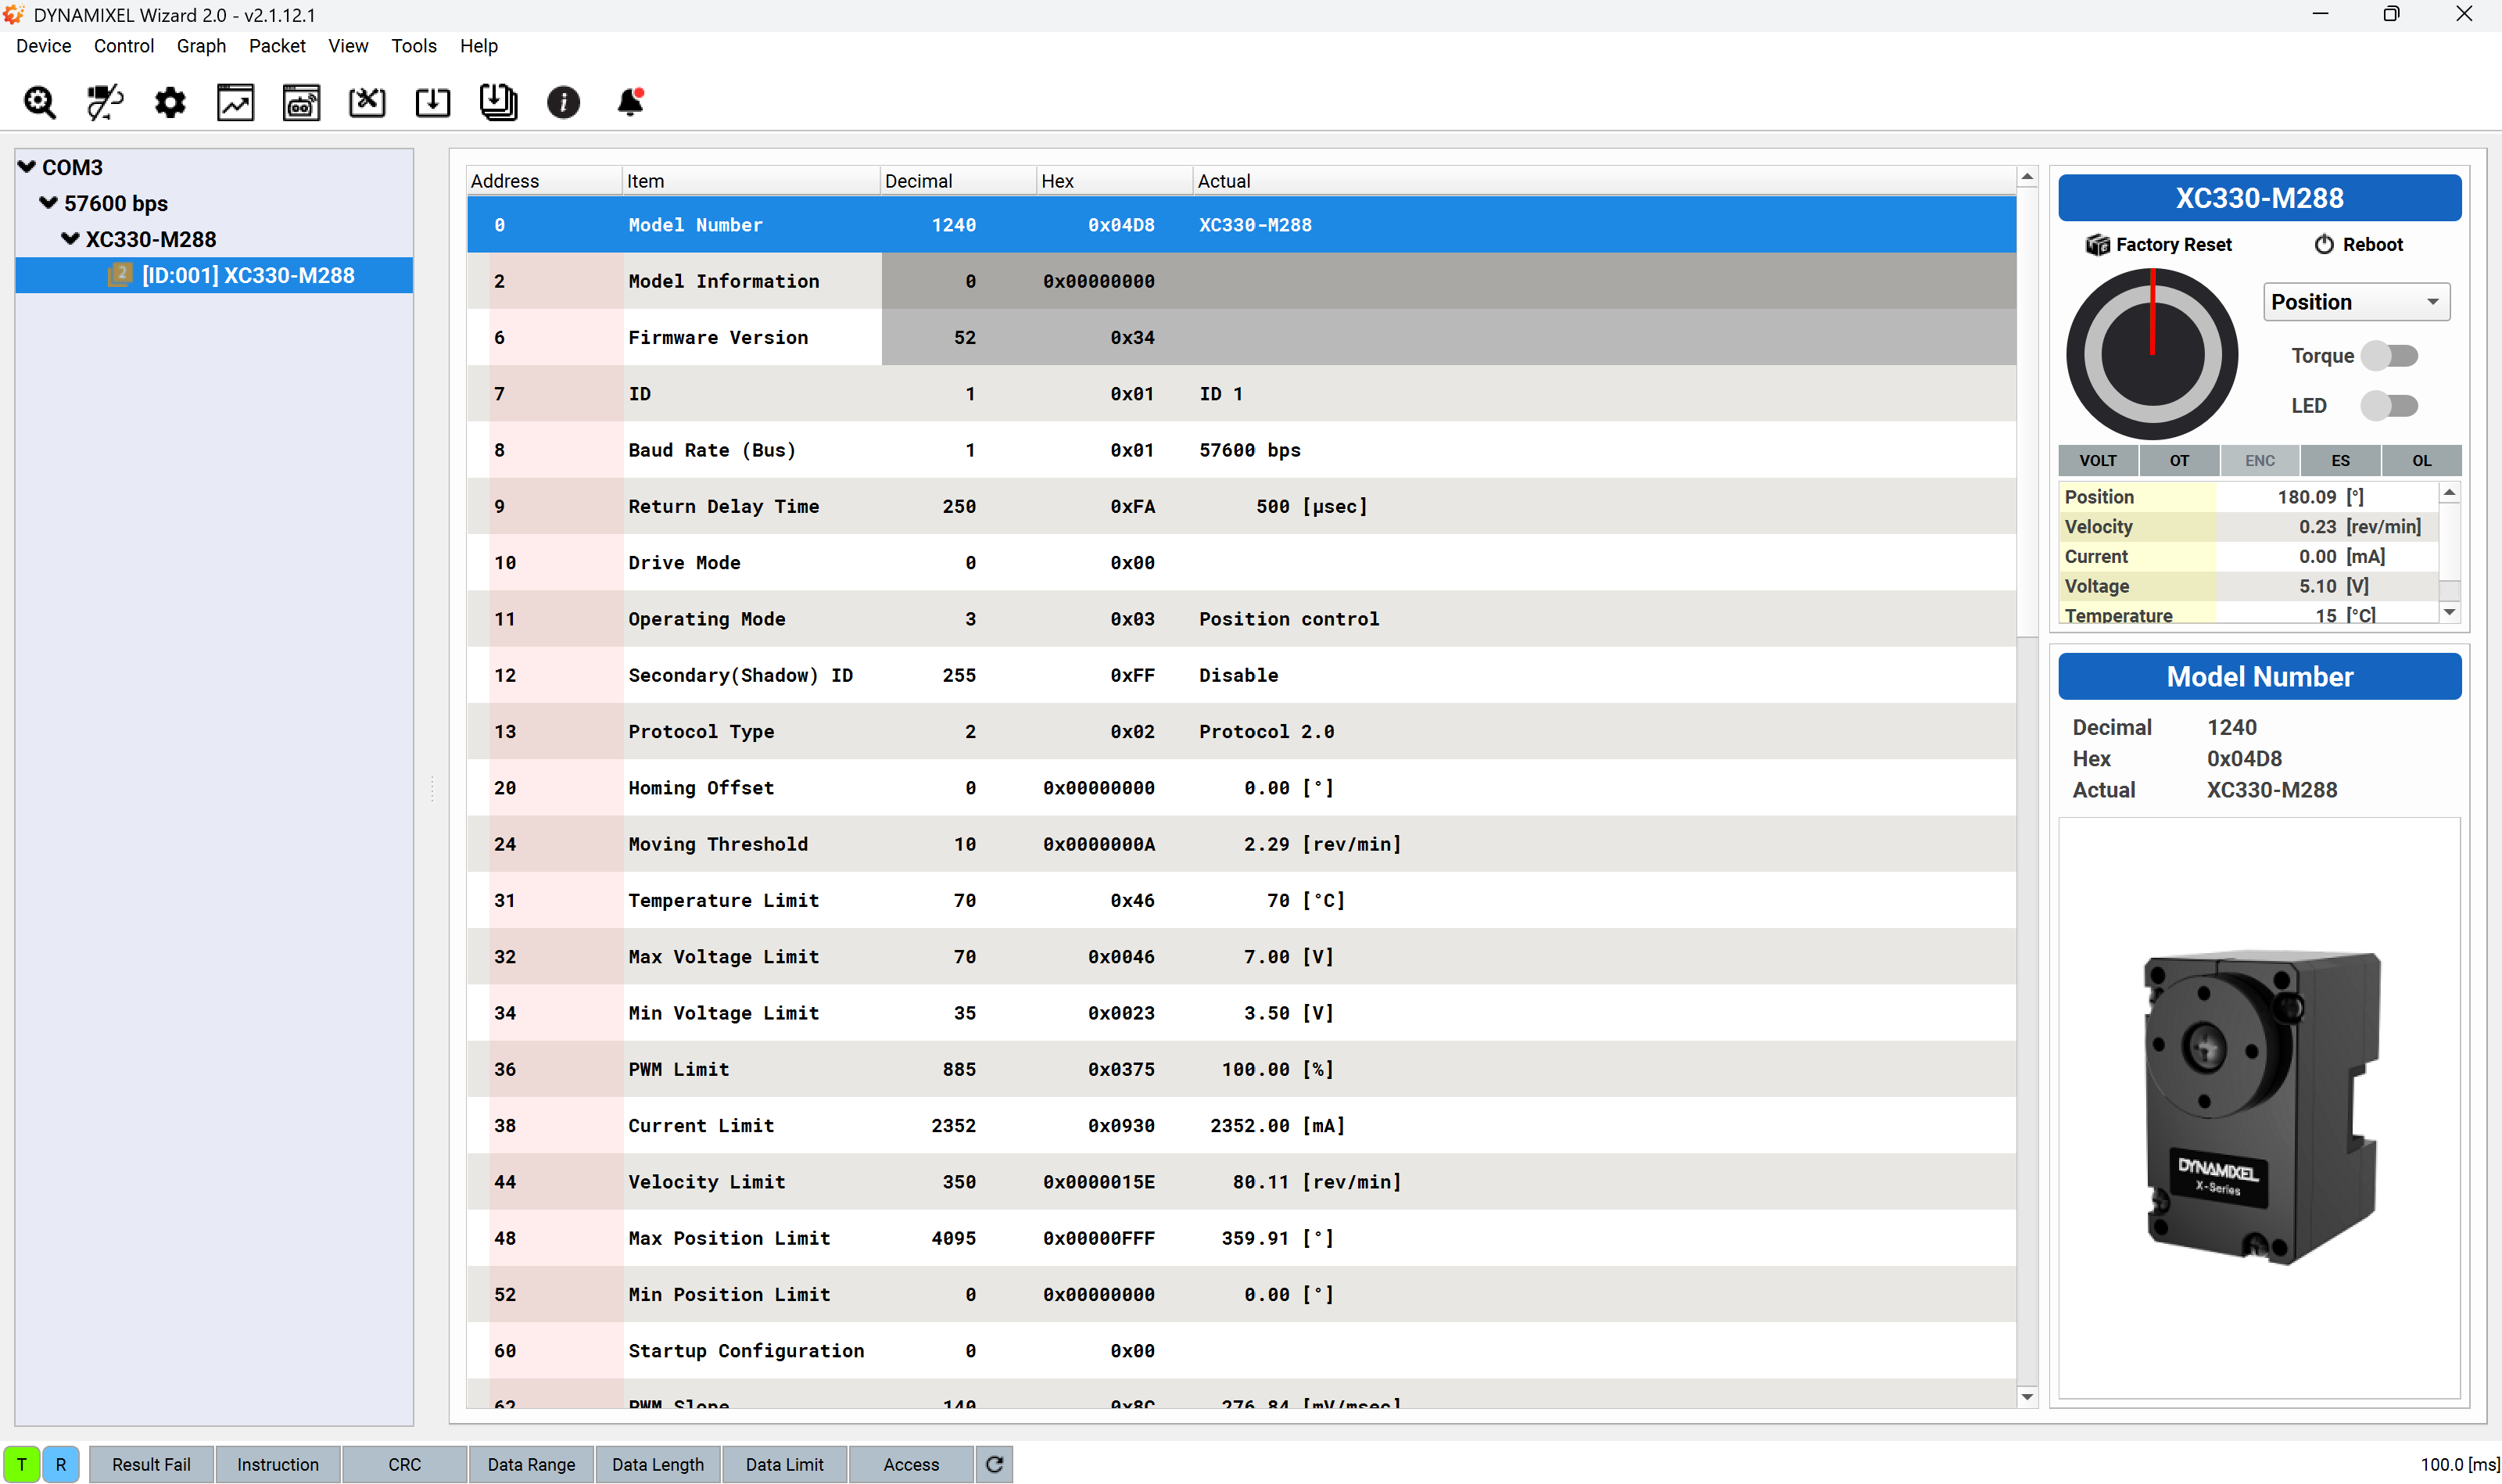
\includegraphics[height=8cm]{figs/chapter3/dynamixel_wizard.png}
    \caption{Interface Gráfica da ferramenta Dynamixel Wizard 2.0 utilizada para alterar o ID de cada motor}
    \label{fig:dynamixel_wizard}
    
\end{figure}


Para além da atribuição de IDs individuais, esta ferramenta permite ainda a definição de grupos de motores com IDs secundários, úteis para cenários em que se pretende acionar vários motores em simultâneo e de forma idêntica. No entanto, esta funcionalidade não será explorada neste projeto, dado que o controlo será efetuado de forma independente para cada atuador.

Adicionalmente, o Dynamixel Wizard 2.0 oferece funcionalidades de diagnóstico e monitorização em tempo real, possibilitando a visualização de parâmetros como a posição atual, velocidade, corrente consumida, entre outros. Esta capacidade é particularmente útil durante as fases de teste, permitindo validar o comportamento dos motores e detetar eventuais anomalias no sistema.

\subsection{Biblioteca Dynamixel SDK}

O Dynamixel SDK é uma biblioteca de software multiplataforma que permite a comunicação e o controlo eficiente dos motores Dynamixel em diversas linguagens de programação, tais como Python, C, C++ e Java. Concebido para proporcionar uma interface unificada e de alto nível, o SDK abstrai as complexidades da comunicação serial, simplificando as operações de leitura e escrita de dados nos motores.

Esta biblioteca suporta os principais protocolos de comunicação Dynamixel, incluindo o Protocolo 2.0, utilizado no presente projeto para os motores XC330-M288-T, o que assegura compatibilidade com as funcionalidades mais recentes dos atuadores, como o controlo de corrente, modos operacionais configuráveis e diagnósticos internos. Através do SDK, é possível configurar parâmetros como posição, velocidade, corrente máxima, limites de movimento e modo de operação, permitindo adaptar o comportamento dos motores às exigências específicas de cada aplicação.

\subsection{ROS2}

O \ac{ROS} é uma \textit{framework} amplamente utilizada no desenvolvimento de sistemas robóticos, proporcionando um ambiente modular que facilita o desenvolvimento, gestão e interligação de múltiplos nós que executam tarefas específicas em paralelo. Esta arquitetura distribuída permite uma organização estruturada do código, promovendo a escalabilidade e a reutilização de componentes, o que é particularmente vantajoso em projetos complexos, como o desenvolvimento de mãos robóticas antropomórficas.

No âmbito da LEAP Hand, Shaw et al. \cite{shaw2023leaphand} disponibilizaram documentação e exemplos compatíveis com Python, ROS 1 e ROS 2, conferindo flexibilidade na escolha da infraestrutura de desenvolvimento. Neste projeto, optou-se pela utilização do ROS 2, em detrimento do ROS 1, com base nas vantagens técnicas e estruturais que a nova versão oferece.

Entre os principais fatores que justificam esta escolha destacam-se a utilização do \textit{middleware \ac{DDS}}, que melhora substancialmente a comunicação entre nós, tornando-a mais eficiente e robusta — um requisito fundamental em sistemas com múltiplos atuadores e sensores a operar em tempo real. Para além disso, o ROS 2 elimina a necessidade de um nó central como o \textit{rosmaster}, permitindo uma arquitetura verdadeiramente distribuída e mais resiliente a falhas. Esta mudança traduz-se numa maior robustez e flexibilidade na gestão da rede de nós, especialmente em contextos com comunicações complexas ou heterogéneas.

Outro fator relevante é o fim gradual do suporte ao ROS 1, cuja manutenção oficial está em fase de descontinuação, sendo que muitas das novas bibliotecas e ferramentas estão a ser exclusivamente desenvolvidas para o ROS 2. A adoção do ROS 2 assegura, portanto, maior longevidade, compatibilidade com futuras atualizações e acesso a funcionalidades mais recentes da comunidade de robótica.

Por fim, o suporte nativo a sistemas real-time, a maior portabilidade entre plataformas e o foco na segurança e escalabilidade reforçam a decisão de utilizar o ROS 2 neste projeto. Esta escolha visa garantir um desenvolvimento mais moderno e sustentável, mantendo a compatibilidade com sistemas robóticos avançados e preparados para integração em ambientes distribuídos.

\subsection{Documentação da LEAP Hand}

Os autores da LEAP Hand \cite{shaw2023leaphand} disponibilizam documentação detalhada e exemplos de código para facilitar a reprodução e o desenvolvimento com base na sua plataforma. Embora essa documentação suporte a utilização em Python, ROS 1 e ROS 2, o código fornecido foi desenvolvido com um foco específico: a execução de políticas previamente treinadas em simulação (utilizando o simulador incluído no projeto) e a realização de movimentos predefinidos da mão robótica.

No entanto, esta abordagem não contempla a possibilidade de controlo direto e individualizado dos motores, nem permite uma personalização completa do comportamento da mão, o que limita a sua aplicabilidade em contextos que exigem maior flexibilidade no desenvolvimento de novos controladores ou algoritmos de manipulação.

Tendo em conta estas limitações, e considerando os objetivos deste projeto, optou-se por não utilizar diretamente o código disponibilizado pelos autores da LEAP Hand, desenvolvendo-se, em alternativa, uma nova infraestrutura de controlo que permite acesso completo e individualizado a cada motor, facilitando o desenvolvimento de estratégias de controlo personalizadas e adaptadas às necessidades específicas deste trabalho.





\section{Conclusão}

Ao longo deste capítulo, foram apresentadas as principais ferramentas de suporte utilizadas no desenvolvimento do projeto, com especial destaque nos componentes de hardware e software que viabilizam a implementação da mão robótica. 

Inicialmente, identificaram-se os motores Dynamixel XC330-M288-T e o controlador U2D2 como soluções adequadas para assegurar movimentos compatíveis com a estrutura da LEAP Hand. A fonte de alimentação foi selecionada com base nas exigências energéticas do sistema, garantindo estabilidade e segurança durante a operação.

Paralelamente, foram descritas as ferramentas de software de apoio à configuração e controlo dos motores, nomeadamente o Dynamixel Wizard 2.0 e a biblioteca Dynamixel SDK, bem como o ambiente de desenvolvimento baseado em ROS 2, que oferece escalabilidade e integração com outros módulos do sistema.

Adicionalmente, a documentação da LEAP Hand foi analisada como referência complementar, optando-se por não utilizar diretamente o código disponibilizado de forma a permitir o controlo individualizado de cada motor.

Em suma, a seleção e integração das ferramentas de suporte descritas neste capítulo estabeleceram uma infraestrutura adaptada às necessidades do sistema, contribuindo para a robustez, modularidade e evolução futura do desenvolvimento da mão robótica.

